\chapter{Use Case 2: FixMyStreet}

% Einführung
\section{Einführung}
FixMyStreet ist ein Konzept, welches bereits in verschiedenen Städten bzw. Ländern umgesetzt wurde. Beispiele dafür sind Deutschland welches dazu die Webseite  \url{http://de.seeclickfix.com/} anbietet oder England mit der Webseite \url{http://www.fixmystreet.com/}. Beide Beispiele bieten neben der Webseite auch native Apps für iOS und Android an.

Die Idee hinter dem Konzept ist so einfach wie auch genial. Man ermöglicht dem Bürger per Webseite oder App entdeckte Defekte in seiner Umgebung (defekte Strassenlampen, Schlaglöcher, usw.) direkt der dafür zuständigen Behörde zu melden. Diese kann dann die erhaltenen Meldungen überprüfen und wenn nötig beheben. So können teure Kontrollfahrten auf ein Minimum reduziert werden.

% Ziel
\subsection{Ziel}
Das Ziel dieses UseCases war die Erstellung einer WebApp, welche genau dieses Konzept umsetzt. Die Benutzer sollen die Möglichkeit haben Defekte in ihrer Umgebung dem zuständigen Amt zu melden.

Google Fusion Table soll dazu als Datenbank verwendet werden, in der die Defekte abgelegt werden. Natürlich sollen auch einige GIS-Features der Fusion Table verwendet werden, um beispielsweise nur die Defekte im aktuell sichtbaren Bereich der Karte zu laden.

% Analyse
\section{Analyse}

\subsection{Storyboard}
Zur Visualisierung der FixMyStreet-Idee wurde vorausgehend ein Storyboard erstellt.

\begin{enumerate}
\item Claudia entdeckt auf ihrem Heimweg eine defekte Strassenlampe \\ 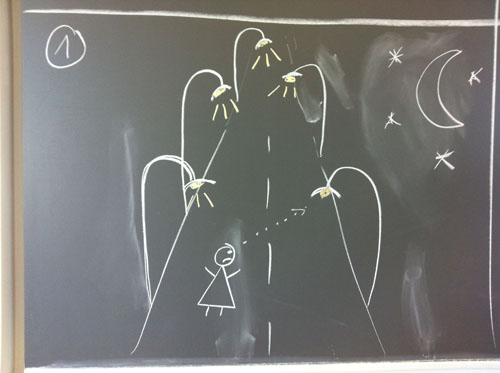
\includegraphics[scale=0.4]{images/usecase2-fixmystreet/storyboard/fixmystreet-storyboard-1.jpg}
\item Sie öffnet die "Fix my street"-App auf ihrem Handy und meldet den Standort der defekten Strassenlampe \\ 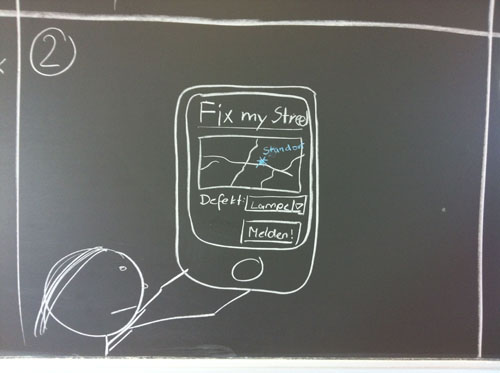
\includegraphics[scale=0.4]{images/usecase2-fixmystreet/storyboard/fixmystreet-storyboard-2.jpg}
\item Am nächsten Tag überprüft der Werkshofleiter Franz die neuen gemeldeten Fälle im System und findet den Eintrag von Claudia \\ 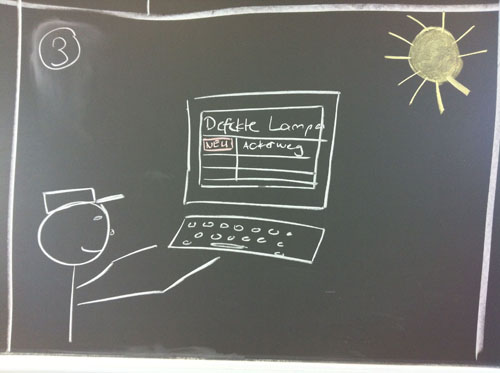
\includegraphics[scale=0.4]{images/usecase2-fixmystreet/storyboard/fixmystreet-storyboard-3.jpg}
\item Er macht sich auf den Weg und repariert die defekte Strassenlampe welche Claudia gemeldet hat \\ 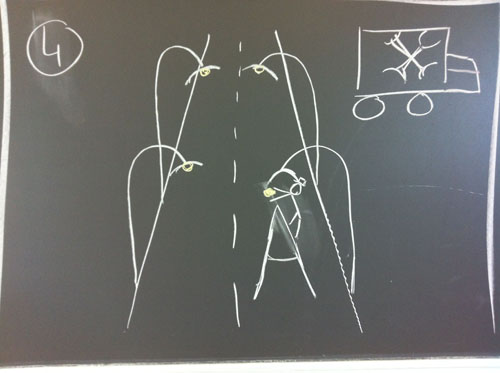
\includegraphics[scale=0.4]{images/usecase2-fixmystreet/storyboard/fixmystreet-storyboard-4.jpg}
\item Am Abend darauf stellt Claudia erfreut fest, dass die Strassenlampe bereits repariert wurde \\ 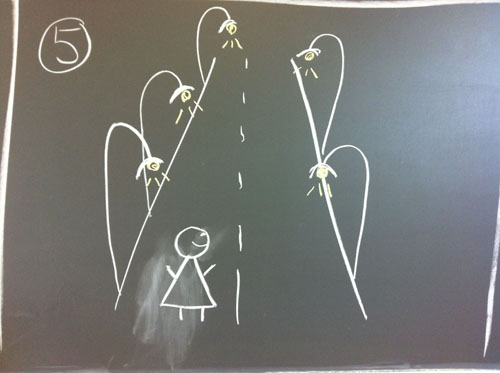
\includegraphics[scale=0.4]{images/usecase2-fixmystreet/storyboard/fixmystreet-storyboard-5.jpg}
\end{enumerate}

\subsection{Use Cases}

\begin{figure}[h!]
	\centering
	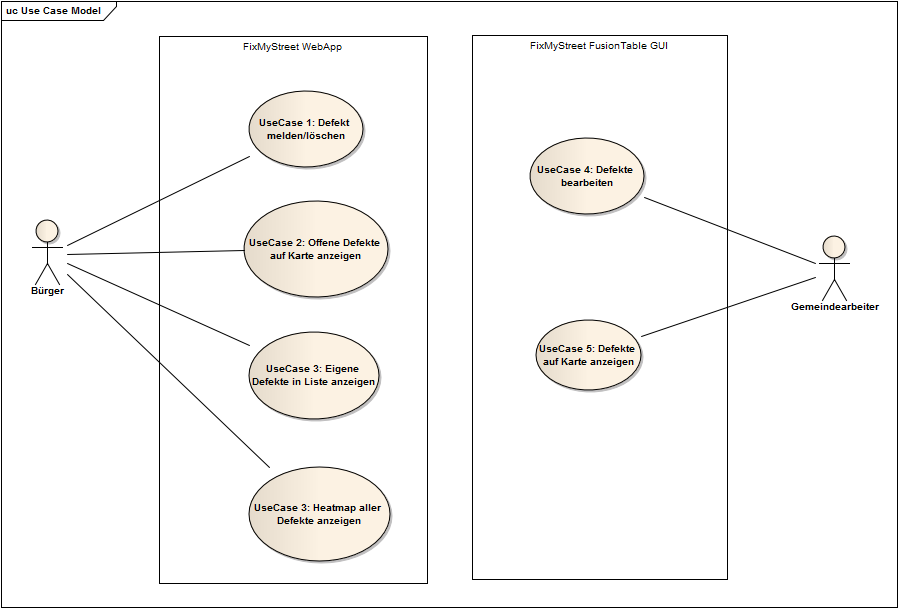
\includegraphics[scale=0.4]{images/usecase2-fixmystreet/uml/fixmystreet-usecasemodel.png}
	\caption{FixMyStreet UseCase Modell}
	\label{fixmystreet-usecasemodel}
\end{figure}

% Use Case 1a: Defekt melden
\subsubsection{Use Case 1a: Defekt melden}
\paragraph{Primary Actor}
\begin{itemize}
\item Bürger
\end{itemize}

\paragraph{Stakeholders and Interests}
\begin{itemize}
\item Bürger: Möchte einen entdeckten Defekt melden
\end{itemize}

\paragraph{Preconditions}
\begin{itemize}
\item WebApp ist gestartet
\end{itemize}

\paragraph{Success Guarantee (Postconditions)}
\begin{itemize}
\item Neuer Defekt ist in Datenbank gespeichert
\item Defekt ist in der Liste und auf der Karte ersichtlich
\item Melde-Maske wurde in den Ursprungszustand zurückgesetzt (kein Defekttyp ausgewählt, Markierung wieder auf die aktuelle Position verschoben)
\end{itemize}

\paragraph{Main Success Scenario}
\begin{enumerate}
\item Bürger wählt Defekttypen aus
\item Bürger verschiebt Markierung auf Karte zur Position des Defekts
\item Bürger sendet den Defekt ab
\item Bürger bestätigt die Kontrollfrage, ob der defekt tatsächlich gesendet werden soll
\end{enumerate}

\paragraph{Alternative Flows}
2a. Markierung muss nicht zwangsläufig verschoben werden. Sie zeigt beim Starten der WebApp auf die aktuelle Position. Falls dies nicht zugelassen wird zeigt sie auf einen vorkonfigurierten Ort.

\paragraph{Special Requirements}
-

\paragraph{Frequency of Occurrence}
Tritt sehr häufig auf, da eine beliebige Anzahl von Bürgern Defekte melden kann.

% Use Case 1b: Defekt löschen
\subsubsection{Use Case 1b: Defekt löschen}
\paragraph{Primary Actor}
\begin{itemize}
\item Bürger
\end{itemize}

\paragraph{Stakeholders and Interests}
\begin{itemize}
\item Bürger: Möchte einen bereits gemeldeten Defekt löschen
\end{itemize}

\paragraph{Preconditions}
\begin{itemize}
\item WebApp ist gestartet
\item Die Listenansicht wurde geöffnet 
\item Es wurde bereits ein Defekt gemeldet
\end{itemize}

\paragraph{Success Guarantee (Postconditions)}
\begin{itemize}
\item Der Defekt wurde aus der Datenbank gelöscht
\item Defekt ist nicht mehr auf der Liste und auf der Karte ersichtlich
\end{itemize}

\paragraph{Main Success Scenario}
\begin{enumerate}
\item Bürger markiert den zu löschenden Defekt in der Liste
\item Bürger wählt den Befehl \emph{Löschen}
\end{enumerate}

\paragraph{Alternative Flows}
2a. Falls der Status des Defektes bereits von einem Gemeindearbeiter geändert wurde (in beispielsweise \emph{In Bearbeitung} oder in \emph{Erledigt}, ist es für den Bürger nicht mehr möglich den Defekt zu löschen.

\paragraph{Special Requirements}
-

\paragraph{Frequency of Occurrence}
Tritt sehr häuft auf, da es für jeden Bürger, welcher bereits einen Defekt gemeldet hat, möglich ist seine eigenen Defekte wieder zu löschen.

% Use Case 2: Noch nicht behobene Defekte auf Karte anzeigen
\subsubsection{Use Case 2: Noch nicht behobene Defekte auf Karte anzeigen}
Der Bürger öffnet die Übersicht. Darin werden ihm alle noch nicht behobene Defekte grafisch auf der Karte angezeigt. Die Daten werden laufend aktualisiert, damit er immer einen aktuellen Stand der Defekte sieht.

% Use Case 3: Heatmap aller Defekte anzeigen
\subsubsection{Use Case 3: Heatmap aller Defekte anzeigen}
Der Bürger öffnet wiederum die Übersicht. Darin hat er die Möglichkeit die Defekte als Heatmap darstellen zu lassen. Dabei werden ihm Gebiete in denen viele Defekte gemeldet wurden farblich stärker markiert als Gebiete in denen kaum Defekte gemeldet wurden. Diese Ansicht wird ebenfalls laufend aktualisiert. 

% Use Case 4: Defekte bearbeiten
\subsubsection{Use Case 4: Defekte bearbeiten}
Der Gemeindearbeiter öffnet die FixMyStreet Google Fusion Table. Darin findet er eine Liste mit allen gemeldeten Defekten. Diese kann er direkt bearbeiten.

\emph{Hinweis: Dieser UseCase wird vom gegebenen Google Fusion Table GUI abgedeckt und wird nicht in der FixMyStreet-App realisiert.}

% Use Case 5: Defekte auf Karte anzeigen
\subsubsection{Use Case 5: Defekte auf Karte anzeigen}
Der Gemeindearbeiter öffnet die FixMyStreet Google Fusion Table. Er hat darin die Möglichkeit alle Defekte auf der Karte anzuzeigen.

\emph{Hinweis: Dieser UseCase wird vom gegebenen Google Fusion Table GUI abgedeckt und wird nicht in der FixMyStreet-App realisiert.}

\subsection{Paper-Prototype}
\paragraph{Maske: Melden}
Auf dieser Maske können Defekte gemeldet werden. Dazu lässt sich zuerst der Defekt-Typ wählen. Danach kann man auf der Karte den Standort des Defekts auswählen indem man die Defekt-Markierung darauf verschiebt. Abschliessend lässt sich die Meldung absenden.

\begin{figure}[!h]
\subfigure[Defekt melden - Übersicht]{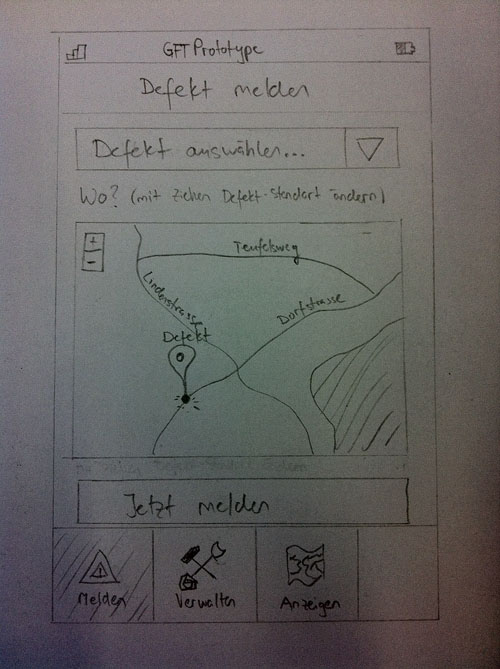
\includegraphics[width=0.45\textwidth]{images/usecase2-fixmystreet/paperprototype/fixmystreet-pp-melden.jpg}}
\hfill
\subfigure[Fehleranzeige beim Absenden ohne Defekttyp-Auswahl]{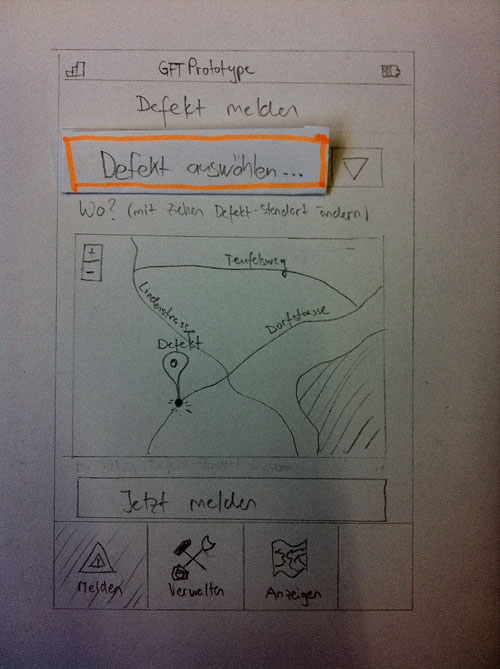
\includegraphics[width=0.45\textwidth]{images/usecase2-fixmystreet/paperprototype/fixmystreet-pp-melden_fehler.jpg}}
\end{figure}

\begin{figure}[!h]
\subfigure[Defekttyp-Auswahl aufgeklappt]{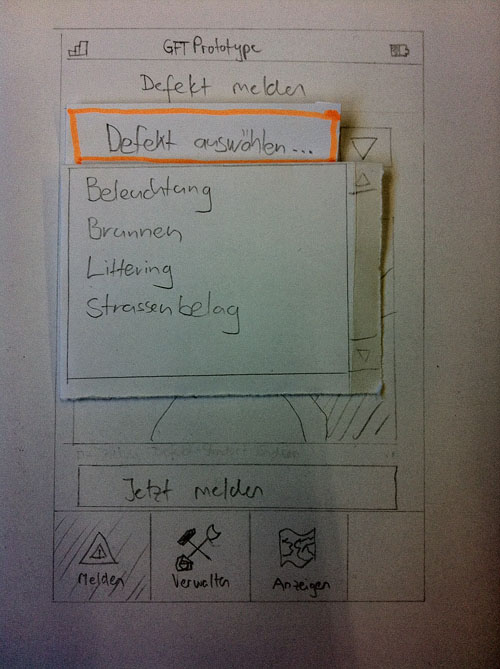
\includegraphics[width=0.45\textwidth]{images/usecase2-fixmystreet/paperprototype/fixmystreet-pp-melden_defektauswaehlen.jpg}}
\hfill
\subfigure[Defekttyp ausgewählt]{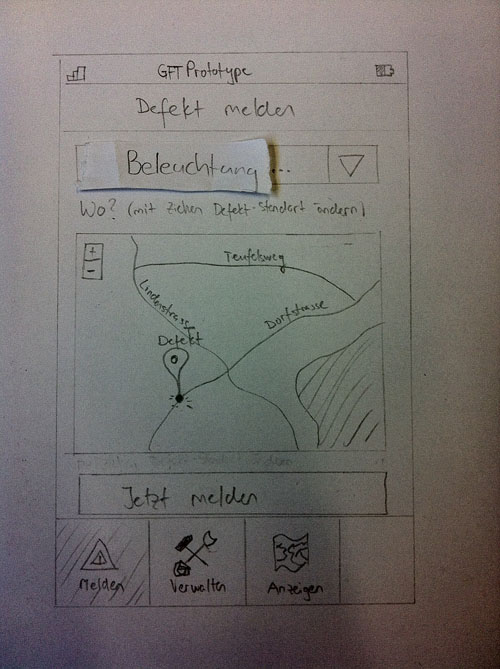
\includegraphics[width=0.45\textwidth]{images/usecase2-fixmystreet/paperprototype/fixmystreet-pp-melden_defektausgewaehlt.jpg}}
\end{figure}

\begin{figure}[!h]
\subfigure[Defekt-Markierung auf Karte verschoben]{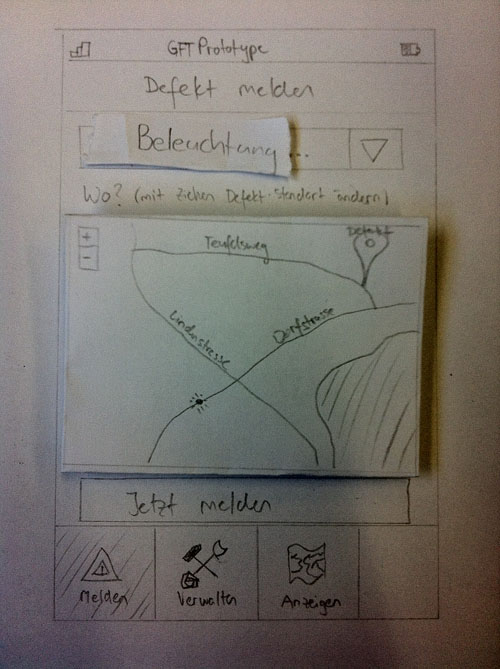
\includegraphics[width=0.45\textwidth]{images/usecase2-fixmystreet/paperprototype/fixmystreet-pp-melden_ortgewaehlt.jpg}}
\hfill
\subfigure[Defekt erfolgreich gemeldet]{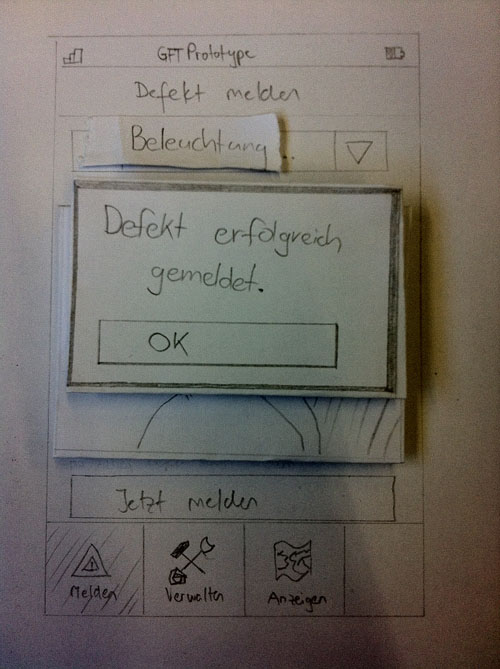
\includegraphics[width=0.45\textwidth]{images/usecase2-fixmystreet/paperprototype/fixmystreet-pp-melden_meldungerfolgreich.jpg}}
\end{figure}

\paragraph{Maske: Verwalten}
In dieser Maske kann man seine eigenen Defekt-Meldungen verwalten. Die gemeldeten Defekte werden gruppiert nach "Offene Defekte" und "Behobene Defekte". Zu jedem Defekt wird der aktuelle Status angezeigt. Mit einem Klick auf einen Defekt erreicht man dessen Detailanzeige.

\begin{figure}[!h]
\subfigure[Defekte verwalten - Übersicht]{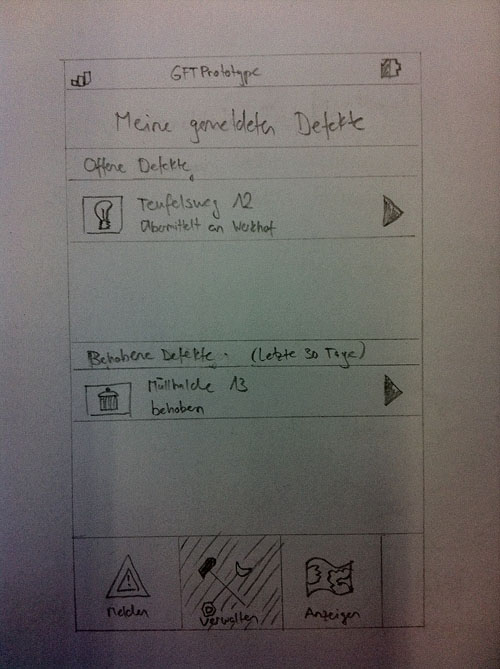
\includegraphics[width=0.45\textwidth]{images/usecase2-fixmystreet/paperprototype/fixmystreet-pp-verwalten.jpg}}
\hfill
\subfigure[Detailansicht eines gemeldeten Defekts]{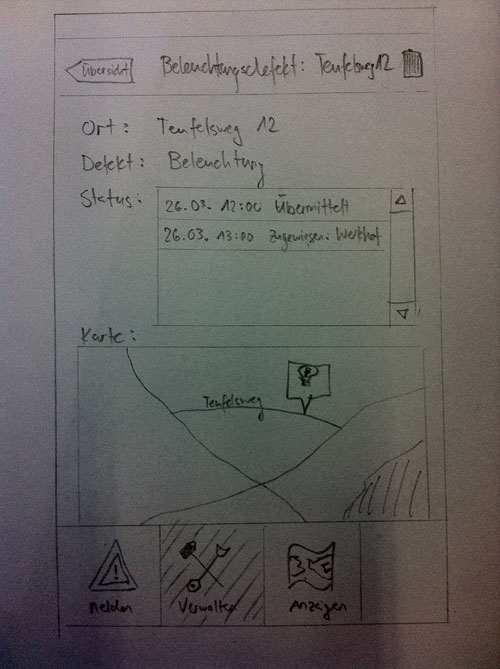
\includegraphics[width=0.45\textwidth]{images/usecase2-fixmystreet/paperprototype/fixmystreet-pp-verwalten_detail.jpg}}
\end{figure}

\paragraph{Maske: Anzeigen}
Auf dieser Maske werden alle gemeldeten Defekte in der Nähe angezeigt. Mit einem Klick auf eine Defekt-Markierung erhält man zusätzliche Information zu diesem Defekt.

\begin{figure}[!h]
\subfigure[Anzeigen - Übersicht]{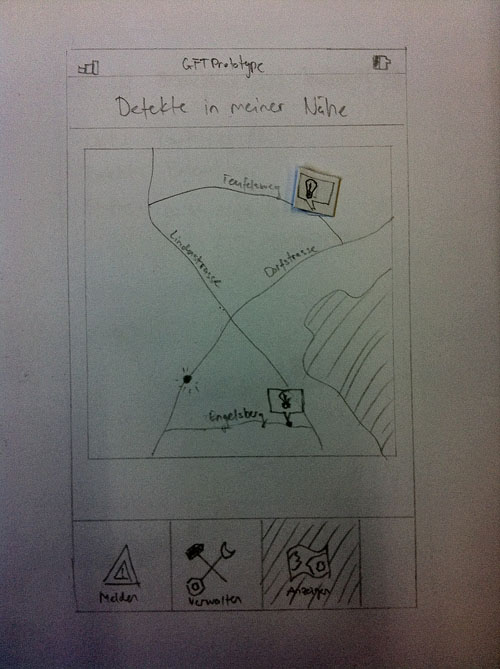
\includegraphics[width=0.45\textwidth]{images/usecase2-fixmystreet/paperprototype/fixmystreet-pp-anzeigen.jpg}}
\end{figure}

% Design
\section{Design}

\subsection{ERD}
Die Applikation verwendet die FusionTable \emph{ftFixMyStreet}. Davon wurden zwei Views erstellt:

\begin{itemize}
\item \emph{ftFixMyStreet\_Read}: In dieser View sind alle Probleme vorhanden. Die Applikation hat aber nur Lesezugriff darauf.
\item \emph{ftFixMyStreet\_Write}: In dieser View sind lediglich die Probleme vorhanden deren Status auf \emph{neu} gesetzt ist. Die Applikation kann darin neue Probleme abspeichern und diese auch wieder löschen.
\end{itemize}

\begin{figure}[h!]
	\centering
	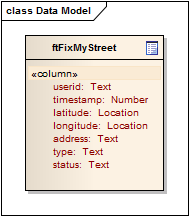
\includegraphics{images/usecase2-fixmystreet/uml/fixmystreet-erd.png}
	\caption{FixMyStreet ERD}
	\label{fixmystreet-erd}
\end{figure}

\subsection{Klassendiagramm}
\todo[inline]{UseCase 2: FixMyStreet - Klassendiagramm}

\subsection{Deploymentdiagramm}

\begin{figure}[h!]
	\centering
	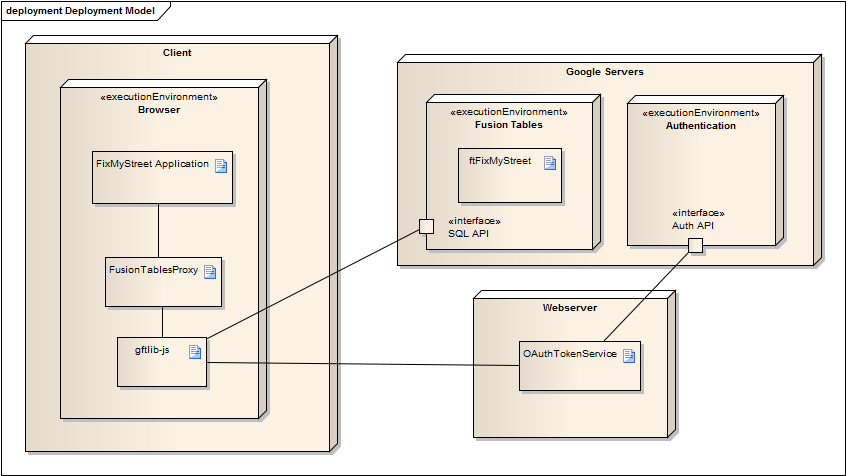
\includegraphics[scale=0.5]{images/usecase2-fixmystreet/uml/fixmystreet-deploymentmodel.png}
	\caption{FixMyStreet Deploymentdiagramm}
	\label{fixmystreet-deploymentmodel}
\end{figure}

\subsection{Starten der Applikation}

\begin{figure}[h!]
	\centering
	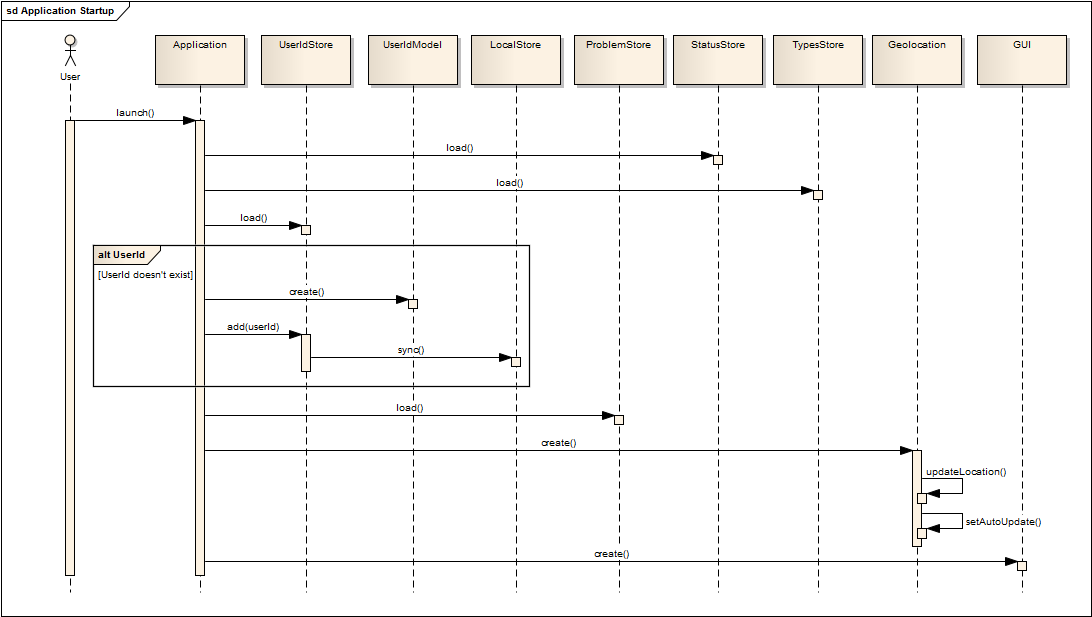
\includegraphics[scale=0.45]{images/usecase2-fixmystreet/uml/fixmystreet-sequencediagram-applicationstartup.png}
	\caption{FixMyStreet Sequenzdiagramm - Starten der Applikation}
	\label{fixmystreet-sequencediagram-applicationstartup}
\end{figure}

% Implementation
\section{Implementation}
\subsection{Systemanforderungen:}
Die WebApp basiert auf dem Sencha Touch 2 Framework. Dieses bietet eine Basis zur Erstellung von mobilen WebApps mit JavaScript. Das Sencha Touch 2 Framework unterstützt alle WebKit-fähigen Browser:

\paragraph{Desktop:}
\begin{itemize}
\item Chrome
\item Opera
\item Safari
\end{itemize}

\paragraph{Mobile:}
\begin{itemize}
\item iOS
\item Android
\item Blackberry
\end{itemize}

\subsection{Abhängigkeiten}
\begin{longtable}{|l|l|p{10cm}|}
\hline 
\textbf{Library} & \textbf{Version} & \textbf{Verwendung} \\ 
\hline 
Sencha Touch 2 & 2.0.1 & Mobile Framework (MVC Applikation) \\ 
\hline 
gftlib-js & 1.0 & Zur Kommunikation mit dem Fusion Table SQL API \\ 
\hline 
jQuery & 1.7.1 & Wird von der gftlib-js verwendet \\ 
\hline 
Google Maps API & V3 & Anzeige der Karten \\ 
\hline 
\end{longtable} 

\section{Implementation}
\subsection{Quellcode-Struktur}

\begin{longtable}{|l|p{9.5cm}|}
\hline 
\textbf{Datei} & \textbf{Beschreibung} \\ 
\hline 
app/app.js & Startet die Applikation \\ 
\hline 
app/controller/List.js & Controller der \emph{List}-View \\ 
\hline 
app/controller/Main.js & Haupt-Controller der Applikation (Steuert die einzelnen Ansichten) \\ 
\hline 
app/controller/Map.js & Basis-Controller der \emph{Report}-View und der \emph{Map}-View \\ 
\hline 
app/controller/ProblemMap.js & Controller der \emph{Map}-View \\ 
\hline 
app/controller/ReportMap.js & Controller der \emph{Report}-View \\ 
\hline 
app/model/*.js & Daten-Modelle der Applikation (Problem, Status, ...) \\ 
\hline 
app/plugin/PullRefresh.js & PullRefresh Plugin der Liste \\ 
\hline 
app/proxy/FusionTables.js & Proxy zur Anbindung der Google Fusion Tabelle an die Applikation \\ 
\hline 
app/store/*.js & Daten-Speicher der Applikation (Probleme, Typen, ...) \\ 
\hline 
app/utli/Config.js & Konfiguration der Applikation \\ 
\hline 
app/utli/Geolocation.js & Steuert Zugriff auf aktuelle Geolocation des Geräts \\ 
\hline 
app/view/*.js & Views der Applikation \\ 
\hline 
resources/images/ & Bilder der Applikation \\ 
\hline 
resources/styles/ & CSS-Styles der Applikation \\ 
\hline 
index.html & Einstiegspunkt der Applikation (Inkludiert app/app.js, welches die Applikation startet) \\ 
\hline
\end{longtable} 

\subsection{Anbindung an Google Fusion Table}
Sencha Touch verwendet für den Zugriff auf fremde Datenquellen das Konzept der Proxies. Ein Proxy verbindet einen internen Applikations-Store mit der eigentlichen Datenquelle.

Es gibt bereits vorgefertigte Proxies, welche die meisten Anwendungsfälle abdecken. So ist es möglich über einen LocalStorage-Proxy mit dem internen Browserspeicher (LocalStorage) zu kommunizieren. Zudem existieren Proxies für AJAX-Serveranfragen oder JSONP-Anfragen.

Für den Zugriff auf die Fusion Table als Datenbank mussten wir aber einen eigenen Proxy schreiben. Dieser verwendet unsere selbst geschriebene Javascript Fusion Table Library \emph{gftlib-js} (siehe Abschnitt \ref{gftlib-js}), um über das SQL API mit der Fusion Table zu kommunizieren.
Der Proxy implementiert lediglich die in unserem UseCase verwendeten CRUD-Operationen Create, Read und Delete. Ein Aktualisieren von gemeldeten Problemen ist über die WebApp nicht vorgesehen und wurde deshalb auch nicht implementiert.
Die Operationen sind jeweils in den Methoden \inlinecode{create()}, \inlinecode{read()} und \inlinecode{destory()} des Proxies abgebildet.

\subsection{Wiedererkennung des Benutzers}
Um die Hemmschwelle zur Benutzung der App möglichst klein zu halten, wollten wir möglichst darauf verzichten, dass sich die Benutzer zuerst Registrieren müssen um die App zu verwenden. Trotzdem soll die App die Möglichkeit haben einen Benutzer wiederzuerkennen, um ihm seine bereits gemeldeten Defekte anzeigen zu können.

Wir generieren dazu beim ersten Starten der App eine Version 1 UUID\footnote{\url{http://de.wikipedia.org/wiki/Universally_Unique_Identifier}} (sequenziell) gemäss RFC 4122\footnote{\url{http://tools.ietf.org/html/rfc4122}}. Diese legen wir im LocalStorage des Browsers ab. Die gemeldeten Probleme beinhalten dann jeweils die UUID und können so den Benutzern zugewiesen werden.

Ein Problem ergibt sich aber aus dieser Vorgehensart. Sobald ein Benutzer seinen Browsercache leert oder die App an einem anderen Gerät startet, erhält er eine neue UUID, welche den neu erfassten Problemen zugeordnet wird. So können verwaiste Datensätze in der Datenbank entstehen, welche keinem Benutzer mehr zugeordnet werden können. In unserem Anwendungsfall ist dies aber nicht weiter schlimm, da die gemeldeten Fälle von der zuständigen Behörde direkt via Fusion Tables GUI bearbeitet werden. Darin spielt die Benutzerzuordnung keine Rolle.

\subsection{Automatisches Aktualisieren der Übersichtsmaske}
Eine weitere Anforderung war es eine möglichst aktuelle Ansicht aller gemeldeten Fälle zu bieten. Wir haben dazu in der Übersichtsmaske ein Polling implementiert. Dieses aktualisiert alle 30 Sekunden die Markierungen auf der Karte indem es eine Anfrage an die Fusion Table sendet. Gelöschte und erledigte Probleme werden entfernt und Neue hinzugefügt.

Die Karte aktualisiert sich zudem jedes Mal, wenn die Übersichtsmaske aufgerufen wird.

\subsection{Auf Übersichtsmaske nur Probleme für sichtbaren Bereich laden}
Um nicht zu viele Markierungen gleichzeitig zu laden und so die Applikation zu verlangsamen, laden wir auf der Übersichtsmaske nur die Probleme, welche im aktuell sichtbaren Bereich der Karte liegen. Sobald die Karte verschoben wird oder der Zoom geändert wird, werden die Probleme für den neuen Bereich nachgeladen.

Dazu haben wir das Spatial-Query \inlinecode{ST\_INTERSECTS} des SQL APIs (siehe Abschnitt \ref{sqlapi-spatialqueries}) verwendet. Als Grenze geben wir ein Rechteck bestehend aus zwei Ecken der momentan angezeigten Karte mit.

\subsection{Heatmap-Ansicht auf Übersichtsmaske}
Auf der Übersichtsmaske hat man die Möglichkeit alle gemeldeten Probleme als Heatmap darzustellen. Dazu haben wir das eine Fusion Table-Ebene über die Karte gelegt und dessen Heatmap-Feature verwendet. 

\section{Test}
\todo[inline]{UseCase 2: FixMyStreet - Test}

\section{Resultate}
Wir hatten einige Probleme bei der Verwendung einer Fusion Table als Datenbank der Applikation. Ein Hauptproblem war klar das Fehlen eines \inlinecode{GRANT}-Mechanismus, wie man ihn von vielen anderen Datenbanksystemen kennt. Die gegebenen Möglichkeiten für die Vergabe von Lese- oder Schreibmöglichkeiten würden für den Gebrauch in einer produktiven Applikation kaum ausreichen.

Zusätzlich konnten wir die GIS-Features, welche Google Fusion Tables anbieten nur minimal nutzen. So hinderte uns die fehlende  Geocodierung von neu eingefügten Datensätzen daran Spatial-Queries zu verwenden (siehe Abschnitt \ref{geocodierung-bug}).

Zudem haben wir bewusst auf die Verwendung einer Fusion Tables-Ebene (siehe Abschnitt \ref{gmap-api-fusiontableslayer}) für die Übersichtsmaske verzichtet, da wir dadurch die Möglichkeit verloren hätten Custom-Markers auf der Karte hinzuzufügen. Dies hätte die Usability der App stark verschlechtert, da man nicht mehr direkt den Typen des markierten Defekts erkannt hätte.

Alles in allem waren die Nachteile bei der Verwendung von Google Fusion Tables als Datenbank wahrscheinlich grösser als deren Vorteile.

\section{Weiterentwicklung}
Auch dieser UseCase hat noch ein grosses Ausbaupotential. So wäre es beispielsweise sinnvoll, wenn man bei der Meldung des Defekts noch ein Foto hinzufügen könnte. Damit könnte man noch genauer zeigen, was wirklich defekt ist. Zudem würde es auch der zuständigen Behörde einfacher fallen Spassmeldungen von echten Defekten zu unterscheiden. Zusätzlich wäre es hilfreich, wenn man die Möglichkeit hätte in einem fakultativen Beschreibungsfeld eine zusätzliche Problembeschreibung anzugeben.

Weiter müssten natürlich auch die Stammdaten (Defekttypen, Status) in eine Datenbank ausgelagert werden. Diese sind momentan statisch im Code verankert. Ein Problem würde sich dabei aber stellen. Das Web-GUI der Fusion Table unterstützt momentan keine Auswahllisten von Daten aus einer fremden Tabelle. Man würde deshalb lediglich die Fremdschlüssel der Stammdaten sehen.

Ein weiteres Feature wäre eine Detailansicht der gemeldeten Probleme. Darin liesse sich der Status-Log anzeigen, um genau nachzuverfolgen, was bereits zur Behebung des angezeigten Defekts unternommen wurde. 

Zudem wäre es sinnvoll, wenn die App auch offline verwendbar wäre. Dadurch könnte man Defekte auch an Orten melden, welche über keine ausreichende Mobilnetzabdeckung verfügen.